\documentclass{standalone}
\usepackage{tikz}
\usetikzlibrary{patterns}
\usetikzlibrary{positioning}
\usetikzlibrary{patterns, positioning}
\usetikzlibrary{shapes.misc}
\usepackage[outline]{contour}
\contourlength{1.5pt} 
\usepackage[sfdefault]{ClearSans}

\begin{document}
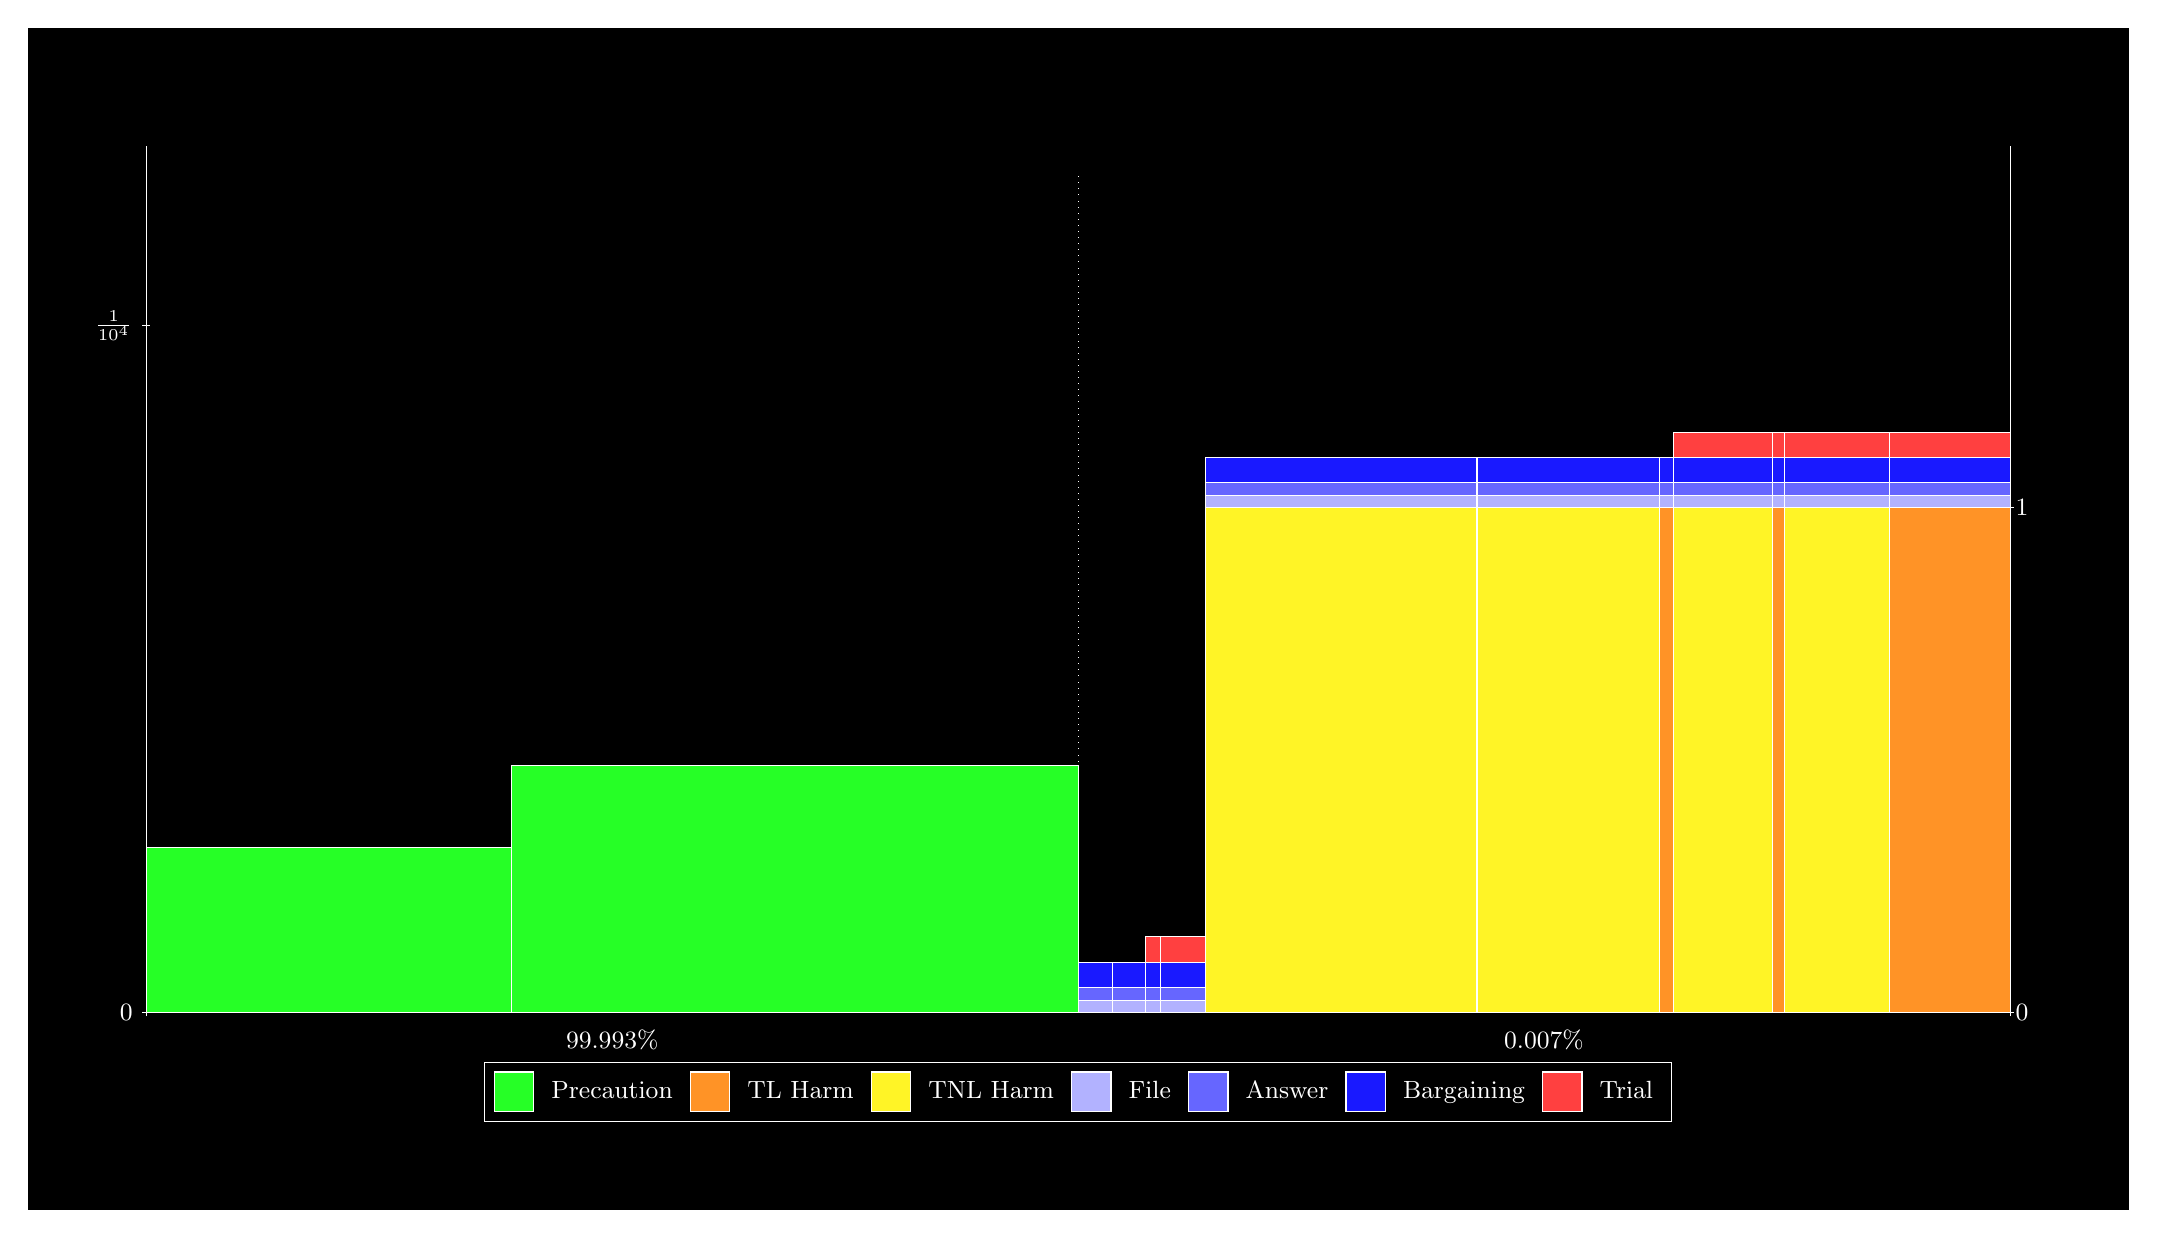
\begin{tikzpicture}
\draw[fill=black] (0,0) rectangle (26.667,15);
\draw[fill=green!85,draw=white,very thin] (1.5,2.5) rectangle (6.1372,4.5941);
\draw[fill=green!85,draw=white,very thin] (6.1372,2.5) rectangle (13.333,5.6412);
\draw[fill=green!85,draw=white,very thin] (13.333,2.5) rectangle (13.772,2.5002);
\draw[fill=blue!30,draw=white,very thin] (13.333,2.5002) rectangle (13.772,2.6604);
\draw[fill=blue!60,draw=white,very thin] (13.333,2.6604) rectangle (13.772,2.8207);
\draw[fill=blue!90,draw=white,very thin] (13.333,2.8207) rectangle (13.772,3.1413);
\draw[fill=green!85,draw=white,very thin] (13.772,2.5) rectangle (14.187,2.5002);
\draw[fill=blue!30,draw=white,very thin] (13.772,2.5002) rectangle (14.187,2.6605);
\draw[fill=blue!60,draw=white,very thin] (13.772,2.6605) rectangle (14.187,2.8208);
\draw[fill=blue!90,draw=white,very thin] (13.772,2.8208) rectangle (14.187,3.1414);
\draw[fill=green!85,draw=white,very thin] (14.187,2.5) rectangle (14.379,2.5002);
\draw[fill=blue!30,draw=white,very thin] (14.187,2.5002) rectangle (14.379,2.6604);
\draw[fill=blue!60,draw=white,very thin] (14.187,2.6604) rectangle (14.379,2.8207);
\draw[fill=blue!90,draw=white,very thin] (14.187,2.8207) rectangle (14.379,3.1413);
\draw[fill=red!75,draw=white,very thin] (14.187,3.1413) rectangle (14.379,3.4618);
\draw[fill=green!85,draw=white,very thin] (14.379,2.5) rectangle (14.944,2.5002);
\draw[fill=blue!30,draw=white,very thin] (14.379,2.5002) rectangle (14.944,2.6605);
\draw[fill=blue!60,draw=white,very thin] (14.379,2.6605) rectangle (14.944,2.8208);
\draw[fill=blue!90,draw=white,very thin] (14.379,2.8208) rectangle (14.944,3.1414);
\draw[fill=red!75,draw=white,very thin] (14.379,3.1414) rectangle (14.944,3.4619);
\draw[fill=green!85,draw=white,very thin] (14.944,2.5) rectangle (18.389,2.5002);
\draw[fill=yellow!85,draw=white,very thin] (14.944,2.5002) rectangle (18.389,8.9114);
\draw[fill=blue!30,draw=white,very thin] (14.944,8.9114) rectangle (18.389,9.0717);
\draw[fill=blue!60,draw=white,very thin] (14.944,9.0717) rectangle (18.389,9.232);
\draw[fill=blue!90,draw=white,very thin] (14.944,9.232) rectangle (18.389,9.5525);
\draw[fill=green!85,draw=white,very thin] (18.389,2.5) rectangle (18.397,2.5002);
\draw[fill=orange!85,draw=white,very thin] (18.389,2.5002) rectangle (18.397,8.9114);
\draw[fill=blue!30,draw=white,very thin] (18.389,8.9114) rectangle (18.397,9.0717);
\draw[fill=blue!60,draw=white,very thin] (18.389,9.0717) rectangle (18.397,9.232);
\draw[fill=blue!90,draw=white,very thin] (18.389,9.232) rectangle (18.397,9.5525);
\draw[fill=green!85,draw=white,very thin] (18.397,2.5) rectangle (20.718,2.5002);
\draw[fill=yellow!85,draw=white,very thin] (18.397,2.5002) rectangle (20.718,8.9115);
\draw[fill=blue!30,draw=white,very thin] (18.397,8.9115) rectangle (20.718,9.0718);
\draw[fill=blue!60,draw=white,very thin] (18.397,9.0718) rectangle (20.718,9.232);
\draw[fill=blue!90,draw=white,very thin] (18.397,9.232) rectangle (20.718,9.5526);
\draw[fill=green!85,draw=white,very thin] (20.718,2.5) rectangle (20.894,2.5002);
\draw[fill=orange!85,draw=white,very thin] (20.718,2.5002) rectangle (20.894,8.9115);
\draw[fill=blue!30,draw=white,very thin] (20.718,8.9115) rectangle (20.894,9.0718);
\draw[fill=blue!60,draw=white,very thin] (20.718,9.0718) rectangle (20.894,9.232);
\draw[fill=blue!90,draw=white,very thin] (20.718,9.232) rectangle (20.894,9.5526);
\draw[fill=green!85,draw=white,very thin] (20.894,2.5) rectangle (22.149,2.5002);
\draw[fill=yellow!85,draw=white,very thin] (20.894,2.5002) rectangle (22.149,8.9114);
\draw[fill=blue!30,draw=white,very thin] (20.894,8.9114) rectangle (22.149,9.0717);
\draw[fill=blue!60,draw=white,very thin] (20.894,9.0717) rectangle (22.149,9.232);
\draw[fill=blue!90,draw=white,very thin] (20.894,9.232) rectangle (22.149,9.5525);
\draw[fill=red!75,draw=white,very thin] (20.894,9.5525) rectangle (22.149,9.8731);
\draw[fill=green!85,draw=white,very thin] (22.149,2.5) rectangle (22.302,2.5002);
\draw[fill=orange!85,draw=white,very thin] (22.149,2.5002) rectangle (22.302,8.9114);
\draw[fill=blue!30,draw=white,very thin] (22.149,8.9114) rectangle (22.302,9.0717);
\draw[fill=blue!60,draw=white,very thin] (22.149,9.0717) rectangle (22.302,9.232);
\draw[fill=blue!90,draw=white,very thin] (22.149,9.232) rectangle (22.302,9.5525);
\draw[fill=red!75,draw=white,very thin] (22.149,9.5525) rectangle (22.302,9.8731);
\draw[fill=green!85,draw=white,very thin] (22.302,2.5) rectangle (23.632,2.5002);
\draw[fill=yellow!85,draw=white,very thin] (22.302,2.5002) rectangle (23.632,8.9115);
\draw[fill=blue!30,draw=white,very thin] (22.302,8.9115) rectangle (23.632,9.0718);
\draw[fill=blue!60,draw=white,very thin] (22.302,9.0718) rectangle (23.632,9.232);
\draw[fill=blue!90,draw=white,very thin] (22.302,9.232) rectangle (23.632,9.5526);
\draw[fill=red!75,draw=white,very thin] (22.302,9.5526) rectangle (23.632,9.8732);
\draw[fill=green!85,draw=white,very thin] (23.632,2.5) rectangle (25.167,2.5002);
\draw[fill=orange!85,draw=white,very thin] (23.632,2.5002) rectangle (25.167,8.9115);
\draw[fill=blue!30,draw=white,very thin] (23.632,8.9115) rectangle (25.167,9.0718);
\draw[fill=blue!60,draw=white,very thin] (23.632,9.0718) rectangle (25.167,9.232);
\draw[fill=blue!90,draw=white,very thin] (23.632,9.232) rectangle (25.167,9.5526);
\draw[fill=red!75,draw=white,very thin] (23.632,9.5526) rectangle (25.167,9.8732);
\draw[white,very thin] (1.5,2.5) -- (1.5,13.5);
\draw[white,very thin] (1.45,2.5) -- (1.55,2.5);
\node[font=\small,text=white, anchor=east] at (1.45, 2.5) {0};
\draw[white,very thin] (1.45,11.226) -- (1.55,11.226);
\node[font=\small,text=white, anchor=east] at (1.45, 11.226) {$\frac{1}{10^{4}}$};

\draw[white,dotted,very thin] (13.333,2.83) -- (13.333,13.17);
\draw[white,very thin] (25.167,2.5) -- (25.167,13.5);
\draw[white,very thin] (25.117,2.5) -- (25.217,2.5);
\node[font=\small,text=white, anchor=west] at (25.117, 2.5) {0};
\draw[white,very thin] (25.117,8.9112) -- (25.217,8.9112);
\node[font=\small,text=white, anchor=west] at (25.117, 8.9112) {1};

\draw[white,very thin] (1.5,2.5) -- (25.167,2.5);
\draw[white,very thin] (1.5,2.45) -- (1.5,2.55);
\node[font=\small,text=white, anchor=north] at (1.5, 2.45) {};
\draw[white,very thin] (25.167,2.45) -- (25.167,2.55);
\node[font=\small,text=white, anchor=north] at (25.167, 2.45) {};

\node[font=\small,text=white,anchor=south] at (7.4167, 1.9) {99.993\%};
\node[font=\small,text=white,anchor=south] at (19.25, 1.9) {0.007\%};
\draw (13.3333,2.5) node (B) {};
\begin{scope}[align=center]
\matrix[scale=0.5,draw=white,below=0.5cm of B,nodes={draw},column sep=0.1cm]{
\node[rectangle,draw,minimum width=0.5cm,minimum height=0.5cm,fill=green!85]{}; & \node[draw=none,font=\small,text=white]{Precaution}; &
\node[rectangle,draw,minimum width=0.5cm,minimum height=0.5cm,fill=orange!85]{}; & \node[draw=none,font=\small,text=white]{TL Harm}; &
\node[rectangle,draw,minimum width=0.5cm,minimum height=0.5cm,fill=yellow!85]{}; & \node[draw=none,font=\small,text=white]{TNL Harm}; &
\node[rectangle,draw,minimum width=0.5cm,minimum height=0.5cm,fill=blue!30]{}; & \node[draw=none,font=\small,text=white]{File}; &
\node[rectangle,draw,minimum width=0.5cm,minimum height=0.5cm,fill=blue!60]{}; & \node[draw=none,font=\small,text=white]{Answer}; &
\node[rectangle,draw,minimum width=0.5cm,minimum height=0.5cm,fill=blue!90]{}; & \node[draw=none,font=\small,text=white]{Bargaining}; &
\node[rectangle,draw,minimum width=0.5cm,minimum height=0.5cm,fill=red!75]{}; & \node[draw=none,font=\small,text=white]{Trial}; \\\\
};\end{scope}

\end{tikzpicture}
\end{document}